\documentclass[tikz,margin=.1in]{standalone}
\usepackage{pgfplots,lmodern}
\pgfplotsset{compat=newest}

\begin{document}
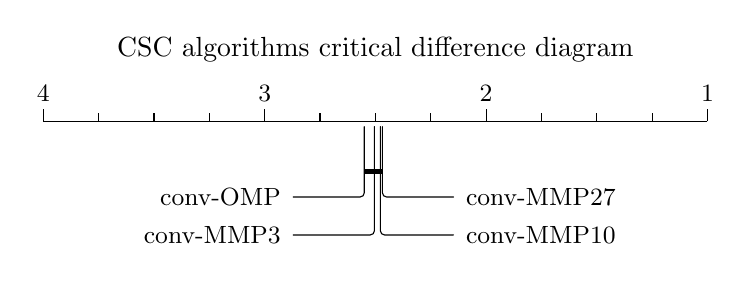
\begin{tikzpicture}[
  treatment line/.style={rounded corners=1.5pt, line cap=round, shorten >=1pt},
  treatment label/.style={font=\small},
  group line/.style={ultra thick},
]

\begin{axis}[
  clip={false},
  axis x line={center},
  axis y line={none},
  axis line style={-},
  xmin={1},
  ymax={0},
  scale only axis={true},
  width={\axisdefaultwidth},
  ticklabel style={anchor=south, yshift=1.3*\pgfkeysvalueof{/pgfplots/major tick length}, font=\small},
  every tick/.style={draw=black},
  major tick style={yshift=.5*\pgfkeysvalueof{/pgfplots/major tick length}},
  minor tick style={yshift=.5*\pgfkeysvalueof{/pgfplots/minor tick length}},
  title style={yshift=\baselineskip},
  xmax={4},
  ymin={-3.5},
  height={4\baselineskip},
  xtick={1,2,3,4},
  minor x tick num={3},
  x dir={reverse},
  title={CSC algorithms critical difference diagram},
]

\draw[treatment line] ([yshift=-2pt] axis cs:2.468125, 0) |- (axis cs:2.1347916666666666, -2.0)
  node[treatment label, anchor=west] {conv-MMP27};
\draw[treatment line] ([yshift=-2pt] axis cs:2.47734375, 0) |- (axis cs:2.1347916666666666, -3.0)
  node[treatment label, anchor=west] {conv-MMP10};
\draw[treatment line] ([yshift=-2pt] axis cs:2.504375, 0) |- (axis cs:2.8834895833333336, -3.0)
  node[treatment label, anchor=east] {conv-MMP3};
\draw[treatment line] ([yshift=-2pt] axis cs:2.55015625, 0) |- (axis cs:2.8834895833333336, -2.0)
  node[treatment label, anchor=east] {conv-OMP};
\draw[group line] (axis cs:2.468125, -1.3333333333333333) -- (axis cs:2.55015625, -1.3333333333333333);

\end{axis}
\end{tikzpicture}
\end{document}
